%\begin{figure}
%\centering
%\includegraphics[width=\columnwidth]{matlab.jpg}
%  \caption{DR-Advisor toolbox for power, price, weather and schedule data capture, baseline prediction, DR policy evaluation and DR synthesis}
%  \label{gui}
%\end{figure}

%DR-Advisor (Figure~\ref{gui}) has been developed into a MATLAB toolbox available at \url{http://mlab.seas.upenn.edu/dr-advisor/}.
In this section, we present a comprehensive case study to show how DR-Advisor can be used to address all the aforementioned demand response challenges (Sec.~\ref{sec:problem}) and we compare the performance of our tool with other data-driven methods. 

\begin{figure}
\centering
\includegraphics[width=0.8\columnwidth]{figs/penn-compressed}
\caption{8 different buildings on Penn campus were modeled with DR-Advisor}
\label{fig:penn}
\end{figure}

\subsection{Building description}
We use historical weather and power consumption data from 8 buildings on the Penn campus (Fig.~\ref{fig:penn}). These buildings are a mix of scientific research labs, administrative buildings, office buildings with lecture halls and bio-medical research facilities. The total floor area of the eight buildings is over 1.2 million square feet spanned across. The size of each building is shown in Tab.~\ref{tab:penn}.

We also use the DoE Commercial Reference Building (DoE CRB) simulated in EnergyPlus as the virtual test-bed building.
This is a large 12 story office building consisting of 73 zones with a total area of 500,000 sq ft. 
There are 2397 people in the building during peak occupancy. 
During peak load conditions the building can consume up to 1.6 MW of power. 
For the simulation of the DoE CRB building we use actual meteorological year data from Chicago for the years 2012 and 2013. 
On July 17, 2013, there was a DR event on the PJM ISO grid from 15:00 to 16:00 hrs. We simulated the DR event for the same interval for the virtual test-bed building.

\subsection{Model Validation}
For each of the Penn buildings, multiple regression trees were trained on weather and power consumption data from August 2013 to  December 2014. 
Only the weather forecasts and proxy variables were used to train the models.
We then use the DR-Advisor to predict the power consumption in the test period \ie for several months in 2015. 
The predictions are obtained for each hour, making it equivalent to baseline power consumption estimate. 
The predictions on the test-set are compared to the actual power consumption of the building during the test-set period. 
%\begin{figure}
%\centering
%\includegraphics[height=3cm, width=\columnwidth]{figs/crbvalid-compressed}
%\caption{Model validation for the clinical research building at Penn.}
%\label{fig:clinical}
%\end{figure}
%One such comparison for the clinical reference building is shown in Figure~\ref{fig:clinical}. 
The following algorithms were evaluated: single regression tree, k-fold cross validated (CV) trees, boosted regression trees (BRT) and random forests (RF).
Our chosen metric of prediction accuracy is the one minus the normalized root mean square error (NRMSE). NRMSE is the RMSE divided by the mean of the data. The accuracy of the model of all the eight buildings is summarized in Tab.~\ref{tab:penn}. We notice that DR-Advisor performs quite well and the accuracy of the baseline model is between 92.8\% to 98.9\% for all the buildings.
\begin{table}
\centering
\caption{Model validation with Penn data.}
%\resizebox{\columnwidth}{!}{%
    \begin{tabular}{l|c|c|c}
    \toprule
    Building Name            & Total Area (sq-ft) & Floors & Accuracy (\%) \\
    \midrule
    LRSM                       & 92,507             & 6      & 94.52       \\
    College Hall               & 110,266            & 6      & 96.40       \\
    Annenberg Center           & 107,200            & 5      & 93.75       \\
    Clinical Research Building & 204,211            & 8      & 98.91       \\
    David Rittenhouse Labs     & 243,484            & 6      & 97.91       \\
    Huntsman Hall              & 320,000            & 9      & 95.03       \\
    Vance Hall                 & 106,506            & 7      & 92.83       \\
    Goddard Labs               & 44,127             & 10     & 95.07   \\
    \bottomrule
    \end{tabular}
 %   }
 \label{tab:penn}   
\end{table}

\subsection{Energy Prediction Benchmarking}
\label{sec:ashrae}
We compare the performance of DR-Advisor with other data-driven method using a bench-marking data-set from the American Society of Heating, Refrigeration and Air Conditioning Engineers (ASHRAE's) Great Energy Predictor Shootout Challenge~\cite{kreider1994predicting}. 
The goal of the ASHRAE challenge  was to explore and evaluate data-driven models that may not have such a strong physical basis, yet that perform well at prediction.
%The competition attracted $\sim150$ entrants, who attempted to predict the unseen power loads from weather and solar radiation data using a variety of approaches.
In addition to predicting the hourly whole building electricity consumption, WBE (kW), both the hourly chilled water, CHW (millions of Btu/hr) and hot water consumption, HW (millions of Btu/hr) of the building was also required to be a prediction output. Four months of training data with the following features was provided: 
\begin{inparaenum}(a)
\item Outside temperature ($^\circ$F)
\item Wind speed (mph)
\item Humidity ratio (water/dry air)
\item Solar flux (W/$m^2$)
\end{inparaenum}
In addition to these training features, we added three proxy variables of our own: hour of day, IsWeekend and IsHoliday to account for correlation of the building outputs with schedule. 

\begin{table}[b!]
\centering
\caption{ASHRAE Energy Prediction Competition Results.}
%\resizebox{\columnwidth}{!}{%
    \begin{tabular}{c|c|c|c|c}
    \toprule
    ASHRAE Team ID & WBE CV & CHW CV & HW CV & Average CV \\
    \midrule
    9              & 10.36  & 13.02  & 15.24 & 12.87      \\
    \textbf{DR-Advisor} & \textbf{11.72}  & \textbf{14.88}  & \textbf{28.13} & \textbf{18.24}     \\
    6              & 11.78  & 12.97  & 30.63 & 18.46      \\ 
    3              & 12.79  & 12.78  & 30.98 & 18.85      \\
    2              & 11.89  & 13.69  & 31.65 & 19.08      \\
    7              & 13.81  & 13.63  & 30.57 & 19.34      \\
    \bottomrule
    \end{tabular}
  %  }
    \label{tab:results}
\end{table}

We use different ensemble methods within DR-Advisor to learn models for predicting the three different building attributes. 
In the competition, the winners were selected based on the accuracy of all predictions as measured by coefficient of variation (CV) statistic. 
The smaller the value of CV, the better the prediction accuracy.
ASHRAE released the results of the competition for the top 19 entries which they received. 
In Tab.~\ref{tab:results}, we list the performance of the top 5 winners of the competition and compare our results with them.
It can be seen from Tab.~\ref{tab:results}, that the random forest implementation in the DR-Advisor tool ranks $2^{nd}$ in terms of WBE CV and the overall average CV. 
%The winner of the competition was an entry from David Mackay~\cite{mackay1994bayesian} which used a particular form of bayesian modeling using neural networks.

The result we obtain clearly demonstrates that the regression tree based approach within DR-Advisor can generate predictive performance that is comparable with the ASHRAE competition winners. 
%Furthermore, since regression trees are much more interpretable than neural networks, their use for building electricity prediction is, indeed, very promising.

\begin{figure}
\subfigure[Rule-based strategies used in DR Evaluation. CHSTP denotes Chiller set point and CLGSTP denotes Zone Cooling temperature set point.]{
\includegraphics[height=6cm, width=0.5\columnwidth]{figs/ControlStrategy-compressed}
\label{fig:case_eval_control}
 }
\subfigure[Prediction of power consumption for 3 strategies. DR Evaluation shows that Strategy 1 (S1) leads to maximum power curtailment.]{
\label{fig:case_eval_power}
\includegraphics[height=6cm, width=0.5\columnwidth]{figs/PowerOutput-compressed}
}
\caption{DR Evaluation.}
\end{figure}

\subsection{DR-Evaluation}
\label{sec:case_eval}

We test the performance of 3 different rule based strategies shown in Fig. \ref{fig:case_eval_control}. 
%The three strategies differ only during the DR Event. 
Each strategy determines the set point schedules for chiller water, zone temperature and lighting during the DR event. 
These strategies were derived on the basis of automated DR guidelines provided by Siemens~\cite{siemensdr}.
%Cooling set point is same in all three cases. 
Chiller water set point is same in Strategy 1 (S1) and Strategy 3 (S3), higher than that in Strategy 2 (S2). Lighting level in S3 is higher than in S1 and S2.
We use auto-regressive trees (Sec.~\ref{sec:autort}) with order, $\delta = 6$ to predict the power consumption for the entire duration (1 hour) at the start of DR Event. In addition to learning the tree for power consumption, additional auto-regressive trees are also built for predicting the zone temperatures of the building.
At every time step, first the zone temperatures are predicted using the trees for temperature prediction. 
Then the power tree uses this temperature forecast along with lagged power consumption values to predict the power consumption recursively until the end of the prediction horizon.

Fig. \ref{fig:case_eval_power} shows the power consumption prediction using the auto-regressive trees and the ground truth obtained by simulation of the DoE CRB virtual test-bed for each rule-based strategy. 
Based on the predicted response, in this case DR-Advisor chooses to deploy the strategy S1, since it leads to the least amount of electricity consumption. The predicted response due to the chosen strategy aligns well with the ground truth power consumption of the building due to the same strategy, showing that DR strategy evaluation prediction of DR-Advisor is reliable and can be used to choose the best rule-based strategy from a set of pre-determined rule-based DR strategies.

\subsection{DR-Synthesis}
\label{sec:case_syn}

 \begin{figure}
\centering
\includegraphics[width=0.78\columnwidth]{figs/newsynth1-compressed}
\caption{DR synthesis using the mbCRT algorithm for July 17, 2013. A curtailment of $380\si{\kilo\watt}$ is sustained during the DR event period.}
\label{fig:synthesis}
\vspace{-10pt}
\end{figure}

We now evaluate the performance of the mbCRT (Sec.~\ref{sec:mbcrt}) algorithm for real-time DR synthesis. 
%Similar to DR evaluation, the regression tree is trained on weather, proxy features, set-point schedules and data from the building. 
We first partition the set of features into manipulated features (or control inputs) and non-manipulated features (or disturbances). 
There are three control inputs to the system: the chilled water set-point, zone air temperature set-point and lighting levels.
At design time, the model based tree built (Algo.~\ref{alg:mbcrt}) has 369 leaves and each of them has a linear regression model fitted over the control inputs with  the response variable being the power consumption of the building.
In addition to learning the power consumption prediction tree, 19 additional model based trees were also built for predicting the different zone temperatures inside the building.
When the DR event commences, at every time-step (every 5 mins), DR-Advisor uses the mbCRT algorithm to determine which leaf, and therefore, which linear regression model will be used for that time-step to solve the linear program \eqref{eq:synth_program} and determine the optimal values of the control inputs to meet a sustained response while maintaining thermal comfort.
% \begin{figure}
%\centering
%\includegraphics[width=\columnwidth]{figs/setpoints-compressed}
%\caption{Optimal DR strategy as determined by the mbCRT algorithm.}
%\label{fig:set-points}
%\vspace{-10pt}
%\end{figure}
%
%\begin{figure}
%\centering
%\includegraphics[width=\columnwidth]{figs/alltemps-compressed}
%\caption{The mbCRT algorithm maintains the zone temperatures within the specified comfort bounds during the DR event.}
%\label{fig:alltemps}
%\vspace{-10pt}
%\end{figure}

\begin{figure*}[b]
\centering
\subfigure[Optimal strategy using mbCRT.]{
\centering
\includegraphics[width=0.48\textwidth]{figs/setpoints-compressed}
\label{fig:set-points}
} \hspace{2pt}
\subfigure[mbCRT maintains thermal comfort.]{
\centering
\includegraphics[width=0.48\textwidth]{figs/alltemps-compressed}
\label{fig:alltemps}
}
\caption{mbCRT DR control strategy and thermal comfort evaluation.}
\end{figure*}

Fig.~\ref{fig:synthesis} shows the power consumption profile of the building using DR-Advisor for the DR event. 
We can see that using the mbCRT algorithm we are able to achieve a sustained curtailed response of $380\si{\kilo\watt}$ over a period of 1 hour as compared to the baseline power consumption estimate.  Also shown in the figure is the comparison between the best rule based fixed strategy which leads to the most curtailment in Section~\ref{sec:case_eval}. In this case the DR strategy synthesis outperforms the best rule base strategy (from Sec.~\ref{sec:case_eval}, Fig.~\ref{fig:case_eval_power}) by achieving a 17\% higher curtailment while maintaining thermal comfort. The rule-based strategy does not directly account for any effect on thermal comfort.
The DR strategy synthesized by DR-Advisor is shown in Fig.~\ref{fig:set-points}. 
We can see in Fig.~\ref{fig:alltemps} how the mbCRT algorithm is able to maintain the zone temperatures inside the building within the specified comfort bounds.
These results demonstrate the benefit of synthesizing optimal DR strategies as opposed to relying on fixed rules and pre-determined strategies which do not account for any guarantees on thermal comfort. 
Fig.~\ref{fig:model-sel} shows a close of view of the curtailed response. The leaf node which is being used for the power consumption constraint at every time-step is also shown in the plot.
We can see that the model switches several times during the event, based on the forecast of disturbances. 
These results show the effectiveness of the mbCRT algorithm to synthesize DR actions in real-time while utilizing a simple data-driven tree-based model.

\subsubsection{\textbf{Revenue from Demand Response}}
We use Con Edison utility company's commercial demand response tariff structure~\cite{edison} to estimate the financial reward obtained due to the curtailment achieved by the DR-Advisor for our Chicago based DoE commercial reference building.
The utility provides a $\$25/\si{\kilo\watt}$ per month as a reservation incentive to participate in the real-time DR program for summer. A payment of \$1 per kWh of energy curtailed is also paid. For our test-bed, the peak load curtailed is $380\si{\kilo\watt}$. If we consider $\sim$5 such events per month for 4 months, this amounts to a revenue of $\sim$\$45,600 for participating in DR which is 37.9\% of the energy bill of the building for the same duration (\$120,317).
This is a significant amount, especially since using DR-Advisor does not require an investment in building complex modeling or installing sensor retrofits to a building.

\subsection{DPC for Peak Power Reduction}
\label{SS:case_dpc}
We next, evaluate the performance of DPCRT (Sec.~\ref{S:control_tree}) for peak power reduction in buildings. This case study is chosen to reflect the advantages of receding horizon control with regression trees to that on one-step look-ahead control as is performed by mbCRT. 
We compare 2 different control algorithms: mbCRT \cite{BehlJainMangharam2016} and DPCRT for peak power curtailment. Recall the model of the building in Sec. \ref{SS:performance_test}. As described before, the data samples consist of 4 types of features, namely weather data, schedule data, building data and autoregressive terms of building power consumption. Of all the features, we use 3 features from the Building Data as controllable variables. These are 
\begin{enumerate}[leftmargin=0.5cm,topsep=1pt,itemsep=-1ex,partopsep=1ex,parsep=1ex]
\item Zone Temperature Cooling Set Point $\mathcal{C}$ [$^{\circ}$C],
\item Chilled Water Temperature Set Point $\mathcal{H}$ [$^{\circ}$C], and
\item Lighting Set Point $\mathcal{L}$ [-].
\end{enumerate}
%\begin{figure}[t]
%\centering
%\begin{tikzpicture}[node distance = 2cm, auto]
%  \node (vd) at (0,0) {\includegraphics[width=20pc]{Figures/scenario2.png}};
%  \coordinate [label=left:16:00] (v) at (1.0,-2.1);
%  \coordinate [label=left:17:00] (v) at (3.85,-2.1);
%  \coordinate [label=right:15:30] (alpha) at (-1.95,-2.1);  
%  \coordinate [label=right:15:00] (alpha) at (-3.85,-2.1);
%  \coordinate [label=right:Peak disturbance] (alpha) at (-1.8,2.3);
%  \coordinate (P) at (-3.6,0);    
%  \draw (P) node[rotate=90] (N) {Power Consumption};
%  \coordinate (Q) at (3.6,0);    
%  \draw (Q) node[rotate=90] (N) {Electricity Price};
%  \draw[stealth-stealth, thick] (-1.5, 2) -- (0.5, 2);
%  \draw[solid, thick] (0.2, 1.85) -- (1.2, 1.85);
%  \draw[solid, thick] (0.2, -1.25) -- (1.2, -1.25);
%  \coordinate [label=right:$30\times$, color=red] (v) at (0.7,0.3);
%  \draw[stealth-stealth, thick] (0.7, 1.85) -- (0.7, -1.25);
%\end{tikzpicture}
%\caption{The test scenario used in the simulations has a $1.5\times$ peak disturbance between 15:30 and 16:00 hrs. The electricity consumption for this peak is typically heavily penalized and is of the order of $30\times$.}
%\captionsetup{justification=centering}
%\label{F:scenario}
%\end{figure}
To predict the power consumption at a future time instance, we first need to predict the zone temperature at that time because they are used as features in the power tree. To accomplish this, two types of trees are built.
\begin{enumerate}[leftmargin=0.5cm,topsep=1pt,itemsep=-1ex,partopsep=1ex,parsep=1ex]
\item Power tree which predicts the power consumption of the building $\mathcal{P}$ using all the features except the controllable features, and
\item Temperature trees which predict the mean zone temperature of each zone. The tree for the $i^{th}$ zone predicts the temperature $\mathcal{T}_i$ using weather data, schedule data and autoregessive terms of the temperature of that zone.
\end{enumerate}
Both the trees use a linear model at the leaves which is a function solely of the controllable variables.
%In the case of mbCRT, we use the formulation \eqref{E:opt_single}, which uses single output regression trees. 
%The objective function $g$ consists of 2 terms: the cost for the power consumption and the cost for the thermal comfort. A factor $\lambda$ is used to trade-off between the two. The optimal control input $\left[  \mathcal{C}^*, \mathcal{H}^*, \mathcal{L}^*  \right]^T $ is determined by solving the following optimization problem at the leaf.
%\begin{align}
%\begin{aligned}
%\text{minimize } \ \ \ & \ \ \ \ \ \ \mathcal{P} + \lambda \sum_i |\mathcal{T}_i - \mathcal{T}_{\mathrm{ref}}| \\ \text{subject to } \ \ \ & \mathcal{T}_i  = \alpha_{0,i} + \alpha_{1,i}\mathcal{C} + \alpha_{2,i}\mathcal{H} + \alpha_{3,i}\mathcal{L} , \\  \ \ \ & \mathcal{P}  = \beta_{0} + \beta_1\mathcal{C} + \beta_2\mathcal{H} + \beta_3\mathcal{L} \\ \ \ \ & \ \ \ \ \ \ \mathcal{C}_{\mathrm{min}} \leq \mathcal{C} \leq \mathcal{C}_{\mathrm{max}}, \\ \ \ \ & \ \ \ \ \ \ \mathcal{H}_{\mathrm{min}} \leq \mathcal{H} \leq \mathcal{H}_{\mathrm{max}}, \\ \ \ \ & \ \ \ \ \ \ \mathcal{L}_{\mathrm{min}} \leq \mathcal{L} \leq \mathcal{L}_{\mathrm{max}}.
%  \end{aligned}
%  \label{E:mbCRT}
%\end{align}
%
For DPC with Regression Trees (DPCRT), we use the formulation \eqref{E:opt_multi2}. Now the objective function covers the cost for the complete horizon. So the governing optimization problem becomes
\begin{align}
\begin{aligned}
\text{minimize } & \sum_{j=1}^p \frac{\mathcal{P}_{\mathrm{j}}^{\mathcal{C}} + \mathcal{P}_{\mathrm{j}}^{\mathcal{H}} + \mathcal{P}_{\mathrm{j}}^{\mathcal{L}}}{3} +  \lambda \sum_{j=1}^p \sum_i \left| \frac{\mathcal{T}_{\mathrm{ij}}^{\mathcal{C}}+\mathcal{T}_{\mathrm{ij}}^{\mathcal{H}}+\mathcal{T}_{\mathrm{ij}}^{\mathcal{L}}}{3} - \mathcal{T}_{\mathrm{ref}} \right| \\ 
\text{subject to } & \ \ \ \mathcal{T}_{\mathrm{ij}}^{\mathcal{C}}  = \alpha_{\mathrm{0,ij}}^{\mathcal{C}} + \alpha_{\mathrm{1,ij}}^{\mathcal{C}} \mathcal{C}_1 + \dots + \alpha_{\mathrm{p,ij}}^{\mathcal{C}} \mathcal{C}_p , \\
\ \ \ & \ \ \ \mathcal{T}_{\mathrm{ij}}^{\mathcal{H}}  = \alpha_{\mathrm{0,ij}}^{\mathcal{H}} + \alpha_{\mathrm{1,ij}}^{\mathcal{H}} \mathcal{H}_1 + \dots + \alpha_{\mathrm{p,ij}}^{\mathcal{H}} \mathcal{H}_p , \\
\ \ \ & \ \ \ \mathcal{T}_{\mathrm{ij}}^{\mathcal{L}}  = \alpha_{\mathrm{0,ij}}^{\mathcal{L}} + \alpha_{\mathrm{1,ij}}^{\mathcal{L}} \mathcal{L}_1 + \dots + \alpha_{\mathrm{p,ij}}^{\mathcal{L}} \mathcal{L}_p , \\
\ \ \ & \ \ \sum_{j=1}^p\mathcal{P}_{\mathrm{j}}^{\mathcal{C}}  = \beta_{\mathrm{0}}^{\mathcal{C}} + \beta_{\mathrm{1}}^{\mathcal{C}} \mathcal{C}_1 + \dots + \beta_{\mathrm{p}}^{\mathcal{C}} \mathcal{C}_p , \\
\ \ \ & \ \ \sum_{j=1}^p\mathcal{P}_{\mathrm{j}}^{\mathcal{H}}  = \beta_{\mathrm{0}}^{\mathcal{H}} + \beta_{\mathrm{1}}^{\mathcal{H}} \mathcal{H}_1 + \dots + \beta_{\mathrm{p}}^{\mathcal{H}} \mathcal{H}_p , \\
\ \ \ & \ \ \sum_{j=1}^p\mathcal{P}_{\mathrm{j}}^{\mathcal{L}}  = \beta_{\mathrm{0}}^{\mathcal{L}} + \beta_{\mathrm{1}}^{\mathcal{L}} \mathcal{L}_1 + \dots + \beta_{\mathrm{p}}^{\mathcal{L}} \mathcal{L}_p , \\
  \ \ \ \ \ & \ \ \ \ \ \ \ \ \ \ \ \ \ \ \mathcal{C}_{\mathrm{min}} \leq \mathcal{C}_j \leq \mathcal{C}_{\mathrm{max}}, \\ 
  \ \ \ \ \ & \ \ \ \ \ \ \ \ \ \ \ \ \ \ \mathcal{H}_{\mathrm{min}} \leq \mathcal{H}_j \leq \mathcal{H}_{\mathrm{max}}, \\ 
  \ \ \ \ \ & \ \ \ \ \ \ \ \ \ \ \ \ \ \ \mathcal{L}_{\mathrm{min}} \leq \mathcal{L}_j \leq \mathcal{L}_{\mathrm{max}}, \\
    \ \ \ \ \ \ \ & \ \ \ \ \ \ \ \ \ \ \ \ \ \ \ \ \ \ j = \left\lbrace 1, \dots, p \right\rbrace.
  \end{aligned}
  \label{E:DPCRT}
\end{align}
Here, the optimization variables are the control inputs for the complete horizon, i.e. $\left[  \mathcal{C}_1, \dots, \mathcal{C}_p  \right]^T $, $\left[  \mathcal{H}_1, \dots, \mathcal{H}_p  \right]^T $ and $\left[  \mathcal{L}_1, \dots, \mathcal{L}_p  \right]^T $.

We now compare the two algorithms when simulated in closed-loop with the EnergyPlus mode of the building. 
The primary difference between mbCRT and DPCRT is that mbCRT is only a single step look-ahead control algorithm while DPCRT is a receding horizon control algorithm. 
In order to compare the performance of DPCRT, we consider a scenario in which there is a significant disturbance which is only anticipated 30 mins in advance and leads to a sudden increase in zone temperatures in the building. This maybe akin to a sunned spike in occupancy or equipment being witched ON at a brief notice.
\begin{figure*}
\centering
\subfigure[Zoomed in view of mbCRT strategy.]{
\centering
\includegraphics[width=0.48\textwidth]{figs/model_switch-compressed}
%\caption{Zoomed in view of the DR synthesis showing how the mbCRT algorithm selects the appropriate linear model for each time-step based on the forecast of the disturbances.}
\label{fig:model-sel}
} \hspace{1pt}
\subfigure[Peak disturbance between 1530-1600 hrs.]{
\includegraphics[width=0.48\textwidth]{figs/peakpowerplot}
\centering
\label{F:scenario}
}
\caption{Left: mbCRT algorithm selects the appropriate linear model for each time-step based on the forecast of the disturbances. Right: The test scenario used in the DPCRT case study simulations has a $1.5\times$ peak disturbance between 15:30 and 16:00 hrs. }
\vspace{-10pt}
\end{figure*}
Under this scenario, it is important to react to the disturbance in a predictive manner in order to minimize the peak power consumption. 
%We test the algorithms on a scenario when there is an unprecedented disturbance which causes a huge peak in the power consumption. 
This scenario is shown in Fig. \ref{F:scenario}. Between 15:30 and 16:00 hrs, an enormous spike in the power consumption ($1.5\times$) is expected because of a scheduled operation.

\begin{figure}[b!]
\centering
\subfigure[Control strategies.]{
\centering
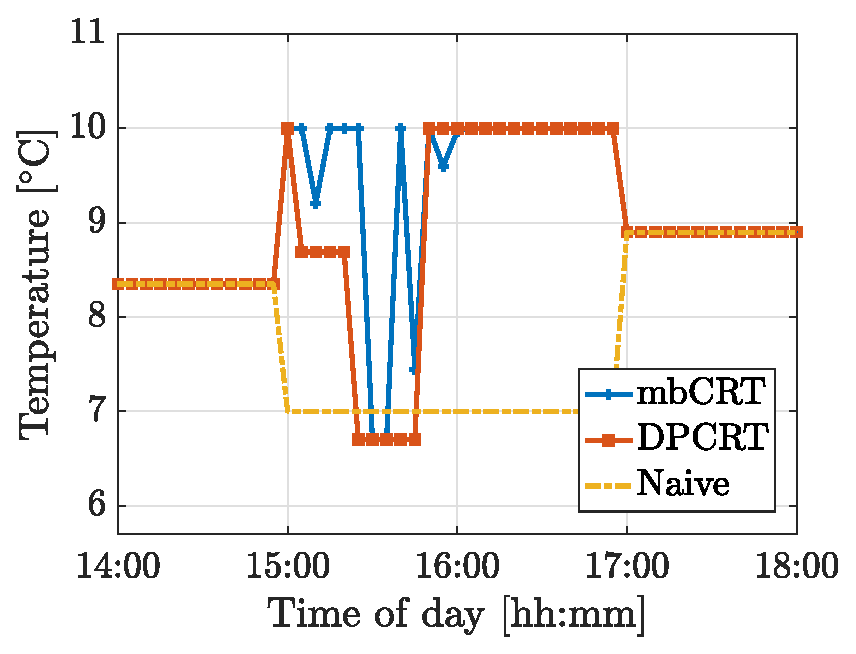
\includegraphics[width=17pc]{Figures/res_control.eps}
\label{F:res_control}
}
\subfigure[Power consumption.]{
\centering
\includegraphics[width=17pc]{Figures/res_power.eps}
\label{F:res_power}
}
\caption{A comparison between mbCRT and DPCRT along with the greedy strategy.}
\captionsetup{justification=centering}
\end{figure}

The control strategies are tested over a 2 hour duration between 15:00 hrs and 17:00 hrs. Fig. \ref{F:res_control} shows 3 control strategies: mbCRT, DPCRT and a Naive load reduction strategy. The naive strategy is equivalent to not responding to the disturbance at all. It maintains the desired zone temeprature set point $\mathcal{C}$, chiller water temperature set point $\mathcal{H}$ and lighting level $\mathcal{L}$ throughout the test period.
In Fig. \ref{F:res_power}, it can be seen that DPCRT reacts to the disturbance much before mbCRT, which waits until the last time-step before the disturbance to react. This leads to a significantly lower peak power consumption that mbCRT.
In the case of DPCRT, the control horizon is 6. 
At 15:00 hrs, DPCRT strategy is same as the greedy one. At 15:05 hrs, the downstream disturbance is visible to DPCRT algorithm and it starts to pre-cool the building by decreasing both cooling and chiller water set points. At 15:25 hrs, the $\mathcal{C}$ and the $\mathcal{H}$ are reduced to mimimum so that in the period of extreme disturbance an optimal trade-off between power consumption and thermal comfort is maintained. Thus, DPCRT algorithm foresees the disturbance and takes a preemptive action against it.  On the other hand, the mbCRT algorithm considers the power consumption and the zone temperatures of only one time step. Therefore, it does not know of an upcoming disturbance. At every time step, it chooses that $\mathcal{C}$, $\mathcal{H}$ and $\mathcal{L}$ which optimizes the cost for that time step. Naturally, this leads to a jaggy behavior in the control strategy.

We can see a similar behavior for the power consumption in Fig. \ref{F:res_power}. The DPCRT algorithm gradually increases the power consumption because it can see the disturbance before it actually reaches 15:30 hrs, while in the case of mbCRT, the power consumption overshoots by a big margin because the controller deals with the disturbance in a single step. DPCRT maintains zone temperature much closer to the reference temperature of 24 degrees while both mbCRT and the naive strategy have large deviations from the desired temperature. 

The quantitative comparison is presented in Tab. \ref{T:case_quant}. Between 15:00 and 17:00 hrs, DPCRT and mbCRT result in similar energy usage, 5102 kWh and 5097 kWh, respectively, both outperforming the Naive strategy which incurs 5358 kWh. Peak power in the case of DPCRT is 1.58 MW which is lower than both mbCRT (1.73 MW) and the Naive strategy (1.63 MW), although Naive outperforms mbCRT. The peak power with DPCRT is 8.6\% less than mbCRT and 3.1\% less than the Naive. While both DPCRT and mbCRT account for thermal comfort, DPCRT deviates less from the desired temperature. The Naive strategy does not trade off on thermal comfort. Thus, DPCRT outperforms mbCRT both in terms of a reduced peak power consumption and better thermal comfort.

%\begin{figure}[t]
%\centering
%\includegraphics[width=20pc]{Figures/res_temp.eps}
%\caption{ Zone temperature of a particular zone under influence of the disturbance.}
%\captionsetup{justification=centering}
%\label{F:res_temp}
%\end{figure}

\begin{table}
  \centering
  \caption{Quantitative comparison for Energy Consumption, Peak Power and \% Reduction in Peak Power of DPCRT compared to Naive approach and mbCRT.}
 % \resizebox{\columnwidth}{!}{
    \begin{tabular}{c|c|c|c}
    \toprule
     & Energy  & Peak Power & Peak \\
     & [kWh] & [MW] & Reduction\\     
    \midrule
    Naive    & 5358  &  1.63 &   3.1\% \\
    mbCRT     & 5097 &  1.73 &   \textbf{8.6\%} \\
    DPCRT     & 5102  &  1.58 &  - \\
    \bottomrule
    \end{tabular}
  %  }
  \label{T:case_quant}
\end{table}
